\documentclass{beamer}
%\documentclass[handout,notes=show]{beamer}
\usetheme{Goettingen}
\newcommand{\bb}[1]{\mathbb{#1}}

\title{Geometric approaches to solving Diophantine equations}
\author[Alex J. Best]{Alex J. Best}
\institute{Tomorrows Mathematicians Today 2013}
\date{16-2-2013}
\DeclareMathOperator{\Vol}{Vol}

\begin{document}

\begin{frame}
\titlepage
\end{frame}

\section{Introduction}
\begin{frame}{Introduction}
Named for Diophantus of Alexandria ($\approx$ 250AD) \\
Some Diophantine equations:
\begin{itemize}
\item<2->{$$x^2 + y^2 = z^2$$ (Pythagorean triples)}
\note{Loads of solutions\\}
\item<3->{$$x^2 - ny^2 = 1$$ (Pell's equation)}
\note{Sometimes solutions\\}
\item<4->{$$x^3 + 48 = y^4$$}
\note{No solutions\\}
\item<5->{$$9^x - 8^y = 1$$}
\note{Only 1 solution\\}
\end{itemize}
\end{frame}

\begin{frame}{What do we want to know?}
\begin{itemize}
\item<2->{Are there any solutions?}\note{We look for solutions in various sets, such as integers or sometimes rationals}
\item<3->{How many are there?}
\item<4->{Can we classify them?}
\item<5->{How can we compute them?}
\end{itemize}
\end{frame}

\begin{frame}{In this talk}
Two general ideas:
\begin{itemize}
\item<2->{Geometry of numbers}
\item<3->{Rational points on surfaces}
\end{itemize}
\end{frame}

\section{Geometry of Numbers}
\begin{frame}{Minkowski and the Geometry of Numbers}
1910 - Hermann Minkowski publishes his paper ``Geometrie der Zahlen'' and sparks a new field called the Geometry of Numbers. \\
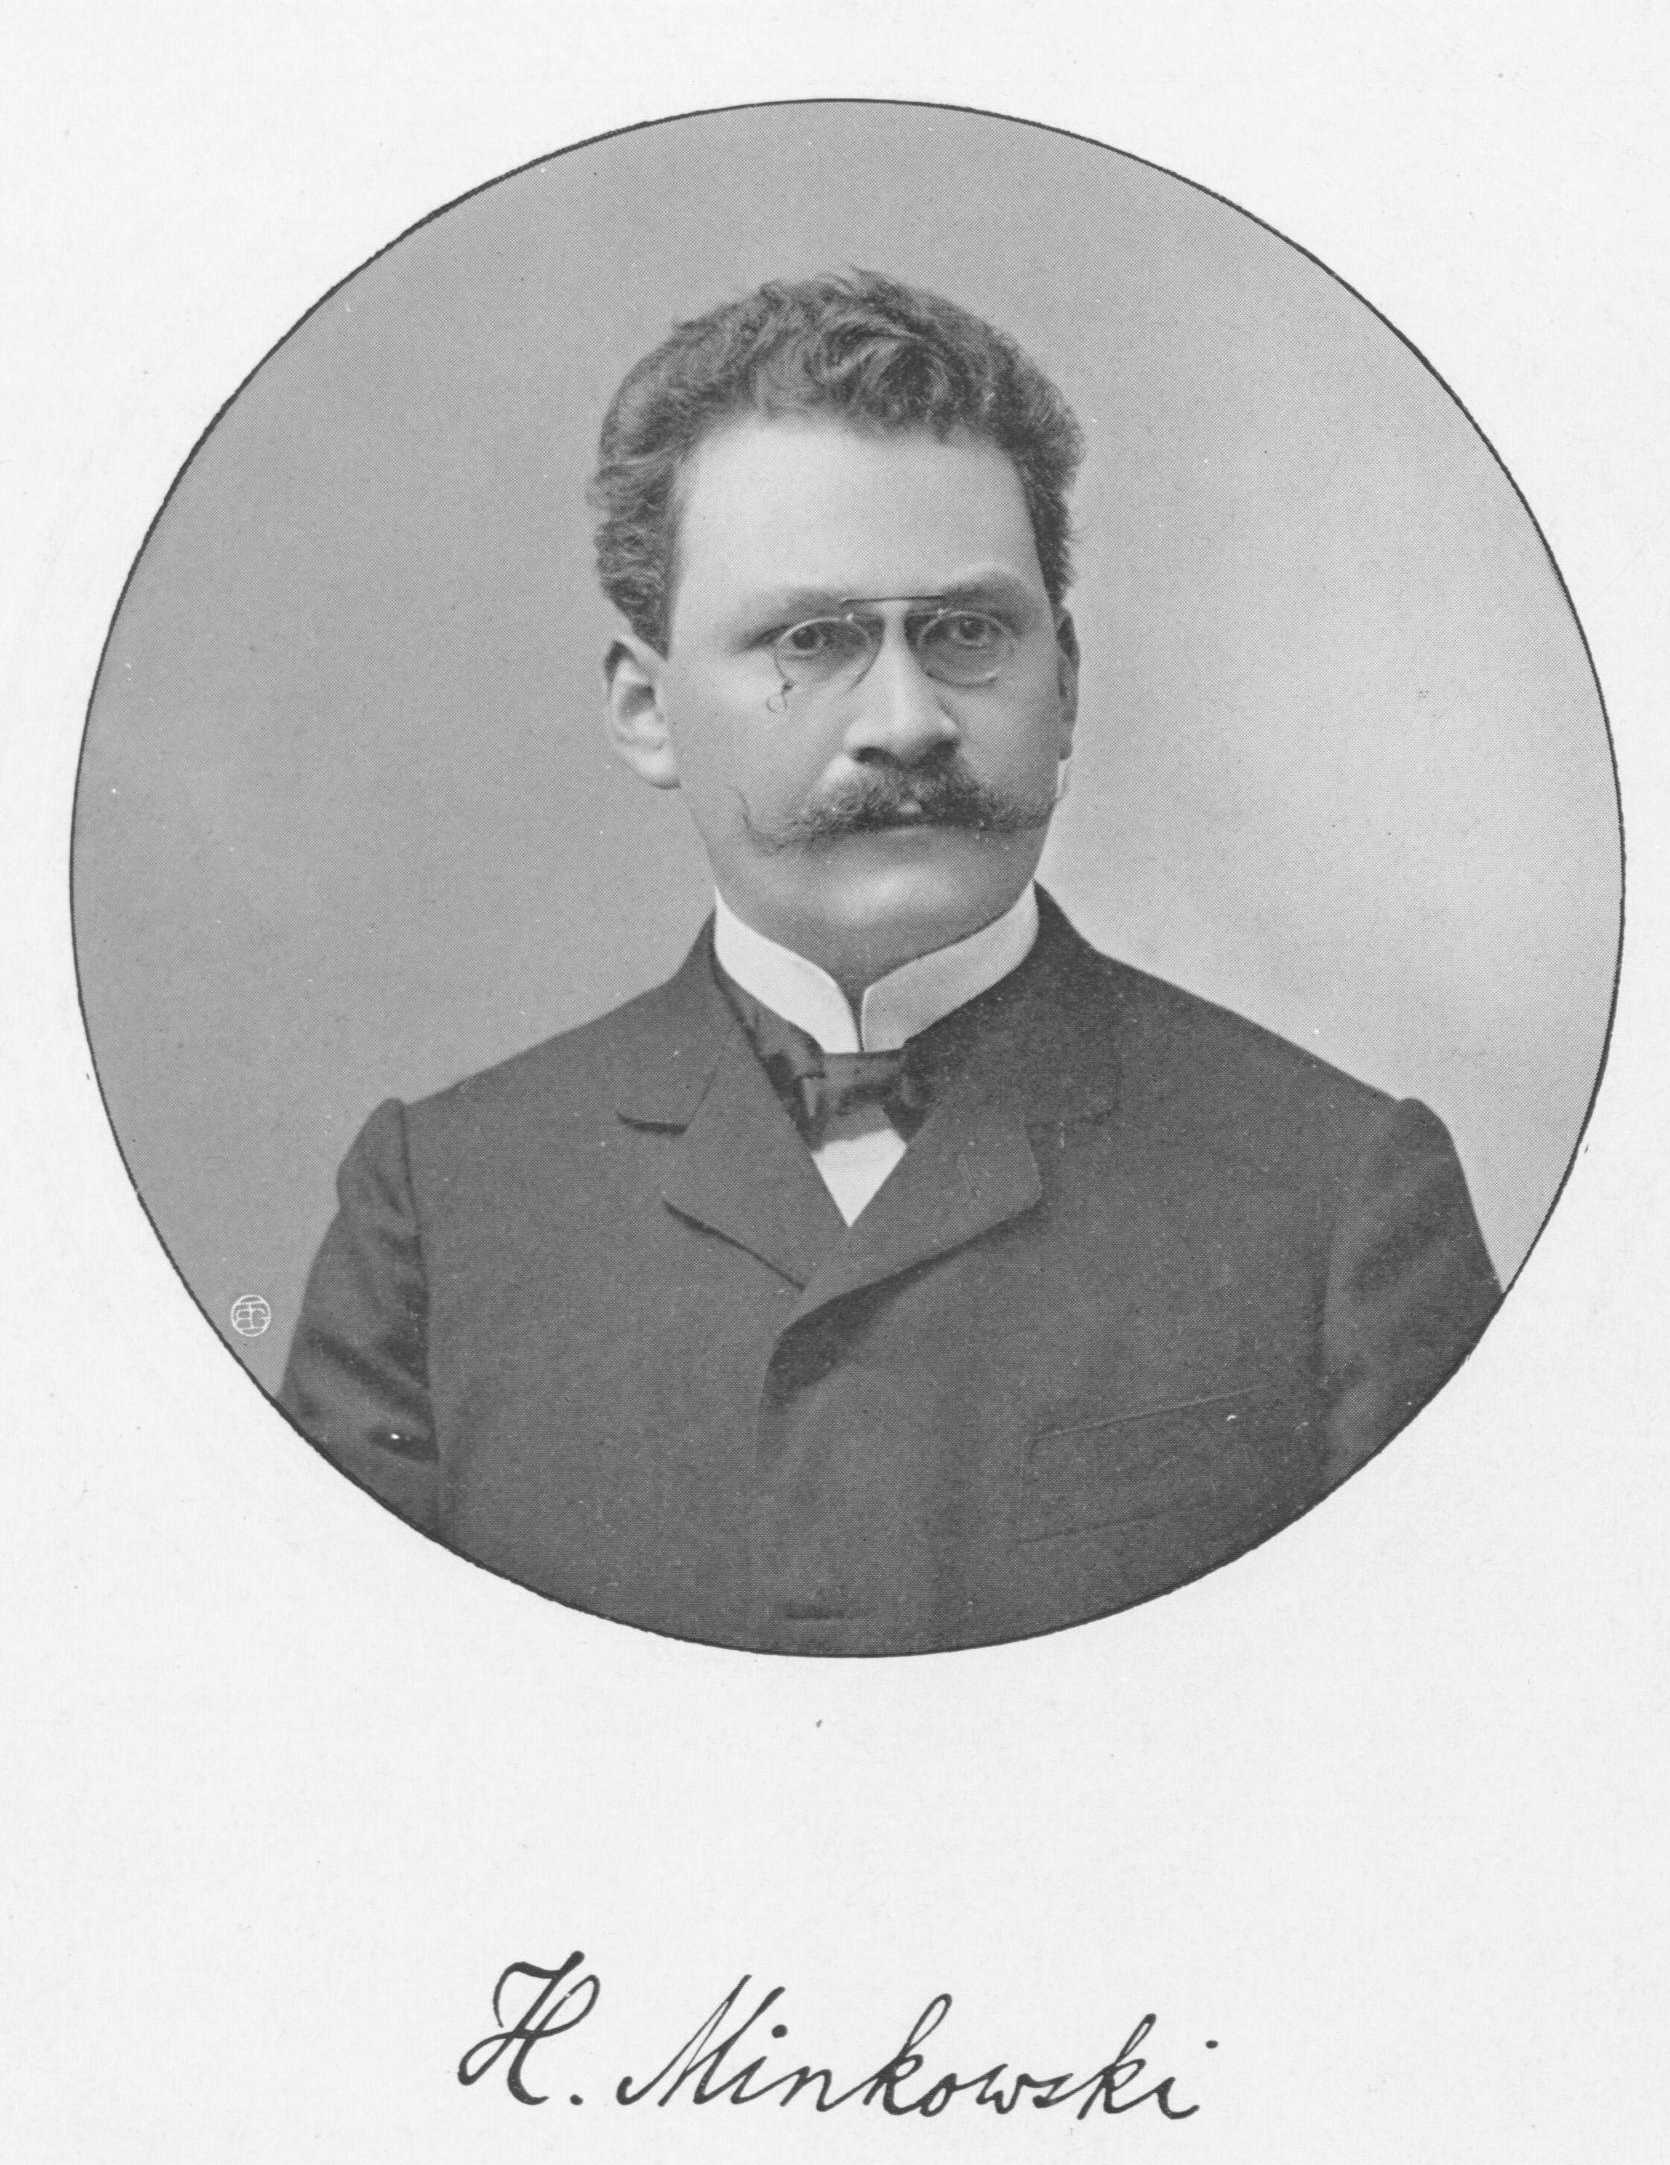
\includegraphics[width=130pt]{img/De_Raum_zeit_Minkowski_Bild}
\quad \quad 
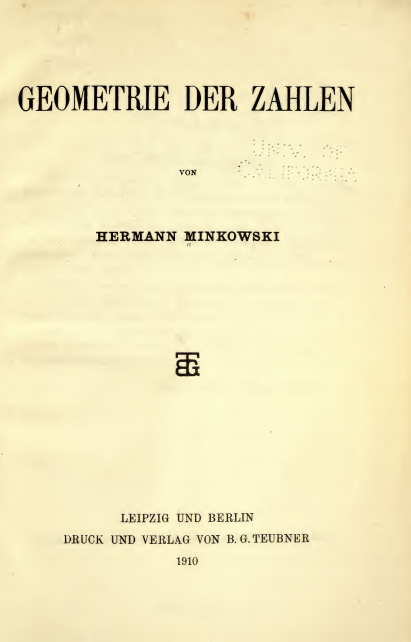
\includegraphics[width=110pt]{img/GeomDerZahlen}
\end{frame}

\note{Cassels intro to geo of numb p.98}
\begin{frame}{A motivating example}
We want to find when integers $x,y$ such that $x^2 + y^2 = p$ where $p$ is prime.\\
\uncover<2->{We can try a few primes, and notice that $2^2+1^2=5$, $3^2+2^2=13$, $4^2+1^2=17$, ... all work.\\}
\uncover<3->{But $7$, $11$, $19$, ... do not.\\}
\uncover<4->{So maybe $x^2 + y^2 = p$ when $p\equiv 1\pmod{4}$.}
\begin{theorem}<4->[Fermat's Christmas Theorem]
An odd prime $p$ can be written as $p = x^2 + y^2$ if and only if $p\equiv 1\pmod{4}$.
\end{theorem}
\end{frame}
\note{Now there are a few different ways of proving this, and Fermat showed it was true long before Minkowski came along}

\begin{frame}{What can geometry do for us?}
\note{$x$ and $y$ are convenient names maybe we could try plotting the points that satisfy our conditions for different p}
When $p=5$ we can look at points satisfying our criteria: \\
\includegraphics<1>[width=0.8\textwidth]{img/sage0}
\includegraphics<2>[width=0.8\textwidth]{img/sage1}
\includegraphics<3>[width=0.8\textwidth]{img/sage2}
\includegraphics<4>[width=0.8\textwidth]{img/sage3}
\end{frame}

\begin{frame}{Minkowski's first theorem}
\note{minkowski's first theorem has a number of forms}
We say a set $B$ in $\bb R^n$ is symmetric if $x\in B \implies -x\in B$. \\
We say a set $B$ is $\bb R^n$ is convex if $x,y\in B \implies x+\lambda (y-x)\in B$ for $0\leq \lambda \leq 1$. \\
\begin{theorem}<2->[Minkowski]
If $B$ is a convex symmetric body and $\Lambda$ a lattice in $\bb R^n$ then $B$ contains a non-zero point of the lattice if:
$$\Vol(B) > 2^di$$
Where $i$ is the area of a single cell of the lattice $\Lambda$.
We can find it using determinants, or the order of our lattice as a subgroup of $\bb Z^n$ for the more algebraically inclined.
\end{theorem}
\end{frame}

\begin{frame}{Let's apply it}
A circle in $\bb R^2$ is symmetric and convex, great!\\
\uncover<2->{The area of our lattice cell is $p$.\\}
\uncover<3->{The area of our circle is $\pi 2p$\\}
\uncover<4->{
So Minkowski tells us that as:
$$\pi 2p = \Vol(B) > 2^di = 2^2p = 4p$$
We have a point which satisfies $x^2 + y^2 = kp$ for some $k \geq 1$, and also $x^2 + y^2 < 2p$.
So $x^2 + y^2 = p$ and we are done.
}
\end{frame}
\note{it surprises me that the fact pi is 3.1415... rather than pi/2 is related to which numbers are expressible as the sum of two squares}

\section{Rational points on surfaces}
\begin{frame}{Rational points on surfaces}
Euler looked at
$$A^4 + B^4 = C^4 + D^4$$
with $A,B,C,D\in\bb Q$ \\
This defines a surface in $\bb R^4$.
\uncover<2->{
%As we only want interesting solutions we take $x = A/D,\ y = B/D,\ z = C/D\in\bb Q$
%}
%\uncover<3->{
%$$\downarrow$$
%$$x^4 + y^4 = z^4 + 1$$
%}
%\end{frame}

%\begin{frame}{Some pictures}
%\includegraphics<1>[width=0.9\textwidth ,trim=0 0 0 150,clip=true]{surface}
%\includegraphics<2>[width=0.9\textwidth ,trim=0 0 0 150,clip=true]{surfacecurve}
%\end{frame}

%\begin{frame}{Parametrisation}
One parametrisation of solutions\cite{hardy}:
$$\begin{array} {lcl}
a(s,t) & = & s^7 + s^5t^2 - 2s^3t^4+3s^2t^5 +st^6 \\
b(s,t) & = & s^6t -3s^5t^2 - 2s^4t^3+s^2t^5 +t^7 \\
c(s,t) & = & s^7 + s^5t^2 - 2s^3t^4-3s^2t^5 +st^6 \\
d(s,t) & = & s^6t +3s^5t^2 - 2s^4t^3+s^2t^5 +t^7 \\
\end{array}$$
}
\uncover<3->{
Unfortunately this does not give us all solutions. 
}
\end{frame}

\begin{frame}{Counting solutions}
Q: How many solutions are there? \\
\uncover<2->{A: $\infty$ \\
Can we find a better way of counting them? \\
We want to estimate the density of our solutions.
}
\end{frame}

\begin{frame}{Heights}
We want a different way of describing the size of a rational number. \\
\note{we could have infinitely many points less than a given bound}
Take
$$x= \frac a b \in \bb Q,\ a,b\in\bb Z$$
$$\gcd(a,b) = 1$$
\uncover<2->{
Then we say height of $x$ is:
$$H(x) := \max\{\log(|a|),\log(|b|)\}$$
}
\uncover<3->{
Hurrah! There are only finitely many points with height less than a given value.
}
\end{frame}

\begin{frame}{Counting points}
We now want to count points in a set $X$ with bounded height.
We do this in a simple way and define:
$$N(X,B) := \#\{x\in X | H(x) \leq B\}$$
We can analyse the growth of this function as $B$ grows.
\uncover<2>{
Manin and others have conjectured that the growth of $N(X,B)$ is asymptotically governed by geometric properties of the surface for many problems\cite{rhb}.
}
\end{frame}

%\begin{frame}{Back to our example}
%We let $S$ be the set of sdfasd and $N(S,B)$ will give us a good idea about how our solutions grow. \\
%\uncover<2>{
%\begin{block} {Manin's conjecture}
%A general conjecture by Manin can be applied which says:
%$$N(S,B) ~ cB(log(B))^k$$
%Where $k,c$ are constants, $k$ is defined by a (complicated) geometric property of the surface.
%\end{block}}
%\end{frame}

\begin{frame}{Morals}
Geometry can help us show solutions exist to Diophantine equations. \\
Geometric properties govern the density of the solutions to some problems. \\
\uncover<2>{And there is a lot more interplay between these two areas.}
\end{frame}

%\begin{frame}{Further reading}
%\note{the extension of these ideas forms a large and rich area known as diophantine geometry}
%\begin{itemize}
%\item<2->{Arithmetic Geometry?!}
%\item<3->{``Diophantine Geometry: An Introduction''}
%\item<4->{Later today: Professor Robin Wilson, ``Leonhard Euler: Life, Labours and Legacy''}
%\end{itemize}
%\end{frame}

\begin{frame}{References}
\begin{thebibliography}{9}

\bibitem{hardy}
  Hardy, G.H. and Wright, E.M. and Heath-Brown, D.R. and Silverman, J.H.,
  An Introduction to the Theory of Numbers,
  Oxford University Press,
  2008.

\bibitem{rhb}
  Heath-Brown, D.R.,
  Diophantine equations, Algebra, Geometry, Analysis \& Logic,
  Talk at Warwick Mathematics Institute.

\end{thebibliography}
\end{frame}
\end{document}
